%!TEX root = ../main.tex

\chapter{Transcription}\label{ch:transcription}

This chapter is dedicated to the problem of offine handwriting recognition, that is, given an image of a text line, find the corresponding characters and words. Although some may consider it a solved task, since many approaches achieve very good performance on a wide variety of corpora (see \autoref{sec:related_transcription}), we remind the reader that our use case poses several challenges that are not present in the controlled environments of academic contests (\autoref{sec:challenges}). Of these, we summarise the most important ones:
\begin{description}
	\item[unbefitting writing conditions] The documents are completed in a rush, soon after an accident, with no proper support structure for writting and with few format restrictions.

	\item[unconstrained recognition] Statements include text which does not admit a vocabulary for correction, such as phone numbers and license plates.

	\item[lack of annotated data] As in the case of detection, we started the project having only a database of images and no useful annotations.
\end{description}

The chapter first introduces the \CRNN{} architecture \citep{CRNN}, which has become almost a standard for optical character recognition in the recent years. Then, \autoref{sec:transcription_experiments} presents several experiments for training, including various methods of data generation. Each new experiment tries to address the weaknesses of the previous one, in a quest of reproducing the great results obtained on clean databases. Finally, we explore the potential of an attention-based architecture coupled with the same training data in \autoref{sec:attention} and present an overview of the obtained results in \autoref{sec:transcription_results}.



%========================================================================================

\section{Convolutional Recurrent Neural Networks}\label{sec:crnn}

	%--INTRO --------------------------------------------------------------------------------

		Text transcription has preoccupied researchers for a very long time. Therefore, a large amount of ideas have been tried in order to solve this problem, of which we mention a few in \autoref{sec:related_transcription}. One of the challenges of text resides in its wide variation of appearance. For example, a free font website such as \url{www.1001fonts.com/} currently lists approximately 9500 different typefaces. Moreover, it is believed that each person has a completely unique handwriting, which is why this is still commonly used a signature. This highlights the importance of being able to represent images of text robustly, or, in other words, to extract good features that distinguish well among characters. As was previously stated, convolutional neural networks have proved very effective in this task time and again, so it is natural to use them as a first stage in a transcription architecture.

		Another peculiarity of text, which we have also mentioned in the detection chapter, is given by its sequential aspect. Few neural network architectures support arbitrarily-sized input. Of these, the recurrent neural network (RNN) has become a standard since it models well sequences of any type.

		The Convolutional Recurrent Neural Network (\CRNN{}) architecture uses the two approaches above in a unified framework to transcribe text from natural images. Considering that it achieved state-of-the-art performance in such a challenging task, we believe it is suitable for our use case as well, which is why we focused most of our efforts in this direction. Next, we detail its inner workings as they are crucial in devising our experiments.


		\begin{figure}
		\begin{subfigure}[c]{.48\linewidth}
		\begin{flushleft}
		\footnotesize
		\begin{tabular}{|l|c|}
			% \footnotesize
			\hline
			\textbf{Type} & \textbf{Configurations}						\tabularnewline	\hline
																																				\hline
			Transcription & - 																\tabularnewline	\hline
			Bi-LSTM & \#hidden units:256						\tabularnewline	\hline
			Bi-LSTM & \#hidden units:256						\tabularnewline	\hline
			Map-to-Seq & - 															\tabularnewline	\hline
			BatchNorm & - 														\tabularnewline	\hline
			Conv (7) & \#maps:512, k:$2\times2$, s:1, p:0	\tabularnewline	\hline
			MaxPool (4) & Window:$1\times2$, s:2								\tabularnewline	\hline
			Conv (6) & \#maps:512, k:$3\times3$, s:1, p:1	\tabularnewline	\hline
			BatchNorm & - 														\tabularnewline	\hline
			Conv (5) & \#maps:512, k:$3\times3$, s:1, p:1	\tabularnewline	\hline
			MaxPool (3) & Window:$1\times2$, s:2 							\tabularnewline	\hline
			Conv (4) & \#maps:256, k:$3\times3$, s:1, p:1	\tabularnewline	\hline
			BatchNorm & - 														\tabularnewline	\hline
			Conv (3) & \#maps:256, k:$3\times3$, s:1, p:1	\tabularnewline	\hline
			MaxPool (2) & Window:$2\times2$, s:2								\tabularnewline	\hline
			Conv (2) & \#maps:128, k:$3\times3$, s:1, p:1	\tabularnewline	\hline
			MaxPool (1) & Window:$2\times2$, s:2 							\tabularnewline	\hline
			Conv (1) & \#maps:64, k:$3\times3$, s:1, p:1		\tabularnewline	\hline
			Input & $W\times32$ gray-scale image 							\tabularnewline	\hline
		\end{tabular}\par
		\caption[\CRNN{} structure]{\todo{Note different from paper, use tabu, split conv part separately }}\label{fig:crnn_architecture}
		\end{flushleft}
		\end{subfigure}
		\begin{subfigure}[c]{.49\linewidth}
			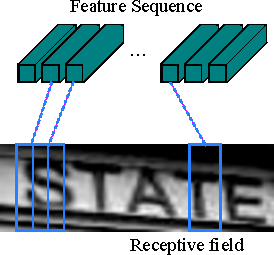
\includegraphics{crnn_rec_field}
			\caption{Image encoding into sequence of features \citep[credit to][]{CRNN}}\label{fig:crnn_sequence}
		\end{subfigure}
		\caption{The \CRNN{} architecture}
		\end{figure}

	%----------------------------------------------------------------------------------------
	\subsection{Feature extraction}
		The first part of the \CRNN{} architecture consists of a custom 7-layer CNN that transforms the input image into a sequence of high-level features. This is similar to well-known architectures, as it alternates convolutional and pooling layers (\autoref{fig:crnn_architecture}). A few particularities are important to be noted.

		First, the input is pooled differently on the vertical dimension than on the horizontal one. For the former, 4 layers with pooling windows of height 2 are used. As a result, an input of height 32 becomes a feature map of height 2. This is further reduced this to a \(\mathit{height} = 1\) feature by the last convolutional layer, which applies \(2 \times 2\) convolution with no padding. For the horizontal direction, the nework performs pooling only twice with a window of width 2. This ensures the receptive field does not become too wide and can still distinguish very narrow characters such as \{\texttt{l,i,1}\}. The network is fully convolutional, which allows inputs of any size to be processed. However, since the columns become features of the RNN, the height should be standardised. This design is well suited for images of text which are bounded vertically, but not horizontally.

		Second, the network uses batch normalisation \citep{batch_norm}, which is standard practice in recent times since it improves the performance and the stability of the network. This works by replacing the activations \(\ve{H}\) of a layer with their normalised counterparts \(\ve{H}'\), which become the new inputs for the next layer: \[
			\ve{H}' = \gamma \frac{\ve{H} - \ve{\mu}}{\ve{\sigma}} + \beta,
		\]\footnote{\todo{make miu and sigma vectors}} where \(\mu\) is a vector of means of all neurons and \(\sigma\) a vector of their standard deviations. The learnable parameters \(\gamma\) and \(\beta\) ensure the network does not lose expressive power by allowing convergence towards any mean and standard deviation. Overall, using this technique means that the composition of the batches is important, as we will see shortly.

		Finally, we use ReLU activations at each layer and bias terms for the convolution.

		%........................................................................................
		\subsubsection*{Input preprocessing}

			Input images are resized to have a heigth of 32px, while keeping their aspect ratio. As a result, their widths are different which makes it difficult to construct batch tensors. Therefore, we also define a standard input width of 250px and make sure all training images are narrower than this in the interest of avoiding horizontal deformation. Images that are shorter than the necessary width are duplicated horizontally up to this size. As opposed to padding the shorter images with blank space, this concatenation mechanism keeps a similar distribution of pixels across all batches. Note this does not produce bad training examples because we keep track of the original length when aligning the predictions and the labels.

	%----------------------------------------------------------------------------------------

	\subsection{RNN decoder}
		The CNN part of the architecture encoded horizontal portions of the image (of full height) into a sequence of high dimensional features, ordered left to right (\autoref{fig:crnn_sequence}). This sequence is then consumed by an RNN decoder in order to produce character representations. To avoid the problem of vanishing gradients in long sequences, the LSTM version is employed \citep{LSTM_original} which uses a combination of gates to control the flow of information inside the cell. By default, an LSTM cell can only use past context in addition to the current input. In our case, future context can be very helpful, so a bi-directional variant of LSTM is used. 	Moreover, using a stack of two such layers allows us to capture more complex contextual dependencies.

		%........................................................................................
		\subsubsection*{Connectionist Temporal Classification}

			Training RNNs normally requires ground truth labels at each time step. We can see this is problematic in our context, since we only know the final sequence and not how it is aligned to the input image. Moreover, some features in the sequence can correspond to space between the characters, so there is no ground truth for them.

			This problem is solved using the Connectionist Temporal Classification method \citep[CTC; ][]{CTC}. It requires the output of the network to be a softmax output layer with \(N + 1\) units, \(N\) being the size of our alphabet \(L\). Each unit represents the probability of a symbol in the alphabet, and the extra unit corresponds to observing no label, which is denoted by ``\(-\)'', a \emph{blank} symbol . In this way, the outputs define the probabilities of all possible alignments of the input sequence with all possible output sequences.

			Additionally, the method requires a many-to-one mapping function from sequences of network outputs, denoted as \(\pi\), to actual labels, denoted as \(\bm l\): \[
				\mathcal{B}: L'^T \to L ^{\leq T},~L' = L \cup \{-\},
			\] where \(L^{\leq T}\) is the set of all possible sequences of length up to \(T\).
	 		For example, \(\mathcal{B}\) maps \mbox{$\pi$: ``\texttt{$-$fee$-$mmm$-$mm$--$ee$-$}}'' to $\bm l$:  ``\texttt{femme}'' by removing duplicates and blanks. Note that the order of these operations is important; removing blanks first results in impossibility of mapping double characters.

	 		Finally, CTC defines the probability of a given label \(\bm{l} \in L^{\leq T}\) conditioned on the input sequence \(\mathbf{x}\) as the sum of the probabilities of all output paths \(\pi\) that correspond to it:
	 		\begin{align*}
				p(\bm{l} | \bm{x}) &= \sum_{\pi:{\cal B}(\pi)=\bm{l}}p(\pi|\bm{x}), \\
				p(\pi | \bm{x}) &= \prod_{t=1}^T \bm{y}_{\pi_t}^{t},
				\label{eq:stringprob}
			\end{align*}
			where \(\bm{y}_{\pi_t}^{t}\) is the probability of observing label \(\pi_t\) at time \(t\), as outputted by the network.

			Given the exponential number of possible sequences \(\pi\) corresponding to \(\bm l\), finding the most probable label \(h(\bm{x}) = \argmax_{\bm{l} \in L^{\leq T}} p(\bm{l} | \bm{x})\) for an input \(\bm x\) becomes intractable very quickly. Therefore, an approximation is made based on the assumption that the most probable path will correspond to the most probable labelling:\[
				h(\bm{x}) \approx \mathcal{B}(\pi^*),~~ \text{where } \pi^* = \underset{\pi}{\argmax}~ p(\pi|\bm{x}).
			\] Decoding in this way can be calculated either with the backward-forward algorithm, or greedily with beam search.

			The loss function between a predicted labelling \(h(\bm{x})\) and a target ground truth label \(\bm z\) is calculated as the edit distance between the two, i.e.\ the number of insertions, deletions or substitutions needed to transform one into the other.

	%----------------------------------------------------------------------------------------

	\subsection{Training and evaluation}
		An input image flows through the convolutional layers and into the LSTM ones, whose predictions are aligned with the ground truth text as explained above. This allows the network to be trained end-to-end on pairs of images and sentences, with the error being back-propagated through all layers. In particular, the LSTM layers use Truncated Back-Propagation Through Time. Also, we noticed improvements when using dropout on the output of the final LSTM with a dropping probability \(p_\mathit{drop} = 0.2\).

		We train the network on batches of 512 images using the Adam optimiser \citep{adam} with a learning rate \(\alpha = 0.001\) and exponential decay rate for the first moment estimates \(\beta_1 = 0.5\). We also tried using an exponentially decreasing learning rate, but found it counter-productive since it needed tuning for each individual corpus or else it would slow down the learning before reaching a plateau.

		Finally, we used an alphabet of 81 characters that we identified in the corpus of the RIMES database: \(2 \times 26\) lower and upper-case letters, 10 digits, 13 French-specific letters with diacritics, and 6 symbols. In addition, we set the architecture to treat as errors differences regarding the case of letters during train time. It is important to note, though, that the distribution of characters in a corpus is not equal, as it is a feature of the language.

		%........................................................................................
		\subsubsection*{Evaluation}
			As in the case of text detection, we started with no ground truth labels on real data. Therefore, to have an objective and relevant measure of the models' performance, we also annotated the bounding boxes of the \ds{Test} dataset. However, the quality for some of these prevented us from providing an accurate transcription. Therefore, we transcribed illegible glyphs with a placeholder character that is not part of the training set. This was done so as to allow wrong predictions at this point while providing normal evaluation for the legible part.

			Given the small size of the \ds{Test} dataset of only 1400 examples, no experiments used it either for training or validation. Each model was only evaluated once on this dataset, and we recorded its performance.

			We use the \emph{normalised} character error rate (CER), and the word error rate (WER) for measuring the performance of different models, expressed as percentages: \[
			\begin{aligned}
				\cer &= \frac{100}{N} \sum_i \frac{\operatorname{dist}(\mathit{prediction}_i, \mathit{groundTruth}_i)}{\card{\mathit{groundTruth}_i}},\\
				\wer &= \frac{100}{N} \sum_i (1 - \delta (\mathit{prediction}_i, \mathit{groundTruth}_i)),
			\end{aligned}
			\]
			where the \(\operatorname{dist}()\) function evaluates the edit distance and \(\delta\) outputs 1 if its arguments are the same, letter for letter, or 0 when they differ. Note that, unless otherwise specified, we use the raw values, without discounting for placeholders in the ground truth. This results in minimally attainable error rates that are slightly above zero: \(\cer_\mathit{min} = 0.8\%,~\wer_\mathit{min} = 5.02\%\).

			Normalising the CER by the length of ground truth is important for aggregating over multiple predictions. Otherwise, mistakes in shorter words would have a heavier contribution than those in longer words. In addition, normalisation also helps in getting an intuitive understanding of the measure; for example, \CER{33} means that one character in three is wrong.

	%----------------------------------------------------------------------------------------

%========================================================================================

\section{Experiments}\label{sec:transcription_experiments}
	Considering the lack of real training data, we try to achieve our goal by the means of transfer learning: we will train our models on several different datasets and evaluate them on real data. The rest of the section presents step-by-step our experiments, describing for each of them the training data, the performance of the model and the identified weaknesses.

	%----------------------------------------------------------------------------------------

	\subsection{Academic databases}
		At the very first phase, we validated that the architecture can learn and perform handwriting recognition by training on the already-discussed RIMES database. We trained and predicted using images of single words, hence the name \ds{Word} model. This converged after seeing \(\approx 780\)k training examples to a \emph{validation} \CER{8.29},	but it did not work on our documents, where \CER{115}. We realised again the importance of pixel values, so we re-trained on \emph{binarised} words, which performed similarly on validation dataset, but had a great improvement on \ds{Test}, with \CER{61.8}. Adding dropout with probability \(p_\mathit{drop} = 0.2\) further lowers the CER by 2\%. Therefore, all further models will use this dropout rate.

		\begin{figure}
			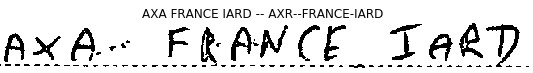
\includegraphics[width=.49\linewidth]{crnn/word_model_3}
			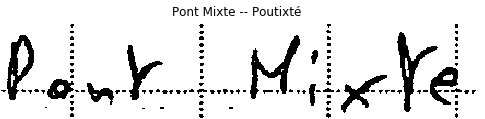
\includegraphics[width=.49\linewidth]{crnn/word_model_1}
			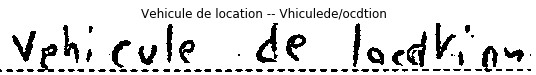
\includegraphics[width=.49\linewidth]{crnn/word_model_2}
			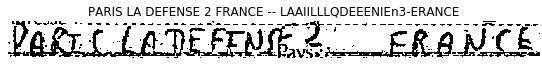
\includegraphics[width=.49\linewidth]{crnn/word_model_4}
			\caption[Predictions of \ds{Words_bin} model]{The ground truth and the predictions are shown above the images (left and right, respectively). When there are few background elements, the prediction works reasonably well, with the exception of missing spaces.}
			\label{fig:crnn_word_drop_model}
		\end{figure}

		While this is far from being usable in practice, the performance improvements demonstrate that transfer learning is a valid strategy, so we continue to explore it. We note that in the examples where the model almost works (\autoref{fig:crnn_word_drop_model}) some of the errors come from the model not being able to predict spaces. This is expected since there are no examples of it in the training set, which contains only images of full words. We try to correct this by including images which contain multiple words. However, we cannot use full lines due to their wildly varying widths, which become a problem for making training batches. Moreover, our cutting algorithm from \autoref{sec:rimes_template} cannot always produce accurate (\texttt{image},\texttt{text}) pairs due to inconsistencies in ground truth data. Therefore, we choose to add those lines from the RIMES database which are narrower than the input width (250px). Given that there are only a few of them, approximately 1000 compared to 50\,000 words, we decide to also add similarly short lines from the IAM handwriting database \citep{iam}, which adds appoximately 2500 examples. With these, together with the words images, we train a new model which again achieves a similarly good performance on its validation dataset. Surprisingly though, it performs much worse on the statements, with a \CER{104}. We believe this is due to the additional English corpus from the IAM database which confuses the language model of the LSTM.

		\subsubsection*{Outcome}
		In general, we validated through many small experiments that it is possible to learn to transcribe handwriting from our corpus by training on a different one. However, the exact composition of the training corpus should be similar to the one of the \ds{Test} dataset at many different levels. First, the pixel distribution has an important role (gray versus binary). Then, the content is important too: we observe a consistent difference between strict and lowercase-only matching (\autoref{tab:transcription_academic}), meaning the model has trouble differentiating the case of words. Finally, the language and the writing style are crucial for the models, since those trained on RIMES+IAM are less stable during training and converge to impractical solutions.

		\begin{table}
			\centering
			\begin{tabular}{| l | *{4}{c |}}\hline
				\textbf{Dataset name} & \textbf{CER strict} & \textbf{CER lower} & \textbf{CER ascii} & \textbf{WER}\\\hline
				\ds{Word} & 115.52 & 109.98 & 109.83 & 98.28\\
				\ds{Word_bin} & 61.43 & 58.44 & 58.43 & 94.25\\
				\ds{Word_bin_drop} & 60.58 & 57.71 & 57.71 & 94.83\\
				\ds{Word_short_IAM} & 104.19 & 100.24 & 100.15 & 98.78\\
				% \ds{Word_short} & 103.70 & 100.97 & 100.74 & 98.71\\
				\ds{Word_short_drop} & 103.77 & 100.36 & 100.17 & 97.70\\\hline
			\end{tabular}
			\caption[Academic datasets results]{Results of the \CRNN{} model trained on different datasets from the academic databases RIMES and IAM. Largely impractical, but useful to confirm the influence of various factors.}\label{tab:transcription_academic}
		\end{table}


	%----------------------------------------------------------------------------------------

	\subsection{Generator}
		Mention problems: writing style, different corpus (MAJ vs min vs ligatures + numbers, plates), lines

		mention the success in OCR

		mention specific changes that we brought (no projection, no curved, random jitter, lines)

		subsubsection: scrapping fonts + elastic distortions

		results:  closer, but not enough doesn't know if it's a date or a number so D, 0, O

				% \ds{Gen_50k} & 67.31 & 63.67 & 63.44 & 93.82\\
				% \ds{Gen_50k_RIM} & 45.78 & 42.06 & 42.13 & 85.78\\
				% \ds{Gen_800f} & 49.02 & 43.98 & 43.66 & 86.21\\
				% \ds{Gen_1M} & 46.06 & 39.85 & 39.55 & 83.62\\
				% \ds{Gen_1M_64} & 50.24 & 43.29 & 42.97 & 85.06\\
				% \ds{Gen_corpus_1} & 47.94 & 40.75 & 40.44 & 81.82\\
				% \ds{Gen_corpus_all} & 49.07 & 40.55 & 40.25 & 82.11\\
				% \ds{Gen_corpus_all*} & 41.76 & 37.03 & 36.70 & 81.11\\
				% \ds{Gen_elastic_1} & 45.14 & 38.59 & 38.30 & 83.33\\
				% \ds{Gen_elastic_2} & 43.97 & 38.95 & 38.70 & 82.90\\
				% \ds{Gen_elastic_3} & 42.20 & 36.92 & 36.64 & 81.68\\
				% \ds{Gen_elastic_4} & 45.29 & 40.16 & 39.89 & 83.41\\

	%----------------------------------------------------------------------------------------

	\subsection{Corpus type}
		strategy 1: precondition the hidden state, like Karpathy
		Not working because not enough information. They were embedding a very rich feature into the space of the hidden state, whereas we merely ``tickle'' the hiddent state

		Strategy 2: add extra feature at all time steps

%========================================================================================

\section{Attention-based architecture}\label{sec:attention}
	biiig TODO

%========================================================================================

\section{Results}\label{sec:transcription_results}

		Show a table of each approach and the corresponding CER, and call it a day :)

\stopToDo{}

